%%%%%%%%%%%%%%%%%%%%%%%%%%%%%%%%%%%%%%%%%%%%%%%%%%%%%
%
%  Template
%  Beamer Presentation by Chris Bourke
%
%%%%%%%%%%%%%%%%%%%%%%%%%%%%%%%%%%%%%%%%%%%%%%%%%%%%%%%%%%%%%%%%%%%%%%%

\documentclass[]{beamer}
%\documentclass[handout]{beamer}

\geometry{papersize={16cm,9cm}}

% For handout version:
%\usetheme[hideothersubsections,slidenumbers]{UNLTheme}
\usetheme[hideothersubsections]{UNLTheme}
\usepackage{amssymb}
\input{StandardCommands}
\usepackage[linesnumbered,ruled,vlined]{algorithm2e}
\SetKwComment{Comment}{//}{}
\DontPrintSemicolon
\SetKwSty{textsc} %
%\SetAlFnt{\scriptsize} %
\SetKwInOut{Input}{Input} %
\SetKwInOut{Output}{Output} %
%\setalcapskip{1em} % changed to
\SetAlCapSkip{1em}
\setlength{\algomargin}{2em} %
%\Setvlineskip{0em} % changed to:
\SetVlineSkip{0em}

\usepackage{tikz}
\usetikzlibrary{fadings}
\usetikzlibrary{shapes.geometric,shapes.symbols}
\usetikzlibrary{calc,shapes.multipart,chains,arrows}
\usetikzlibrary{arrows.meta,calc,shapes.multipart,chains,arrows}
%\usetikzlibrary{calc,shapes.multipart,chains,arrows}
%%\usetikzlibrary{backgrounds}
\usetikzlibrary{backgrounds}
\usetikzlibrary{decorations.pathreplacing}
\usetikzlibrary{decorations.pathmorphing}
\tikzset{onslide/.code args={<#1>#2}{%
  \only<#1>{\pgfkeysalso{#2}} % \pgfkeysalso doesn't change the path
}}
\tikzset{temporal/.code args={<#1>#2#3#4}{%
  \temporal<#1>{\pgfkeysalso{#2}}{\pgfkeysalso{#3}}{\pgfkeysalso{#4}} % \pgfkeysalso doesn't change the path
}}

\tikzset{
    fading speed/.code={
        \pgfmathtruncatemacro\tikz@startshading{50-(100-#1)*0.25}
        \pgfmathtruncatemacro\tikz@endshading{50+(100-#1)*0.25}
        \pgfdeclareverticalshading[%
            tikz@axis@top,tikz@axis@middle,tikz@axis@bottom%
        ]{axis#1}{100bp}{%
            color(0bp)=(tikz@axis@bottom);
            color(\tikz@startshading)=(tikz@axis@bottom);
            color(50bp)=(tikz@axis@middle);
            color(\tikz@endshading)=(tikz@axis@top);
            color(100bp)=(tikz@axis@top)
        }
        \tikzset{shading=axis#1}
    }
}

\usepackage{multirow}
\usepackage{multicol}

\definecolor{steelblue}{rgb}{0.2745,0.5098,0.7059}
\hypersetup{
    colorlinks = true,
    urlcolor = {steelblue},
    linkbordercolor = {white}
}

\definecolor{mintedBackground}{rgb}{0.95,0.95,0.95}
\definecolor{mintedInlineBackground}{rgb}{.90,.90,1}

%\usepackage{newfloat}
\usepackage{minted}
\setminted{mathescape,
               linenos,
               autogobble,
               frame=none,
               fontsize=\small,
               framesep=2mm,
               framerule=0.4pt,
               %label=foo,
               xleftmargin=2em,
               xrightmargin=0em,
               startinline=true,  %PHP only, allow it to omit the PHP Tags *** with this option, variables using dollar sign in comments are treated as latex math
               numbersep=10pt, %gap between line numbers and start of line
               style=default, %syntax highlighting style, default is "default"
               			    %gallery: http://help.farbox.com/pygments.html
			    	    %list available: pygmentize -L styles
               bgcolor=mintedBackground} %prevents breaking across pages
               
\setmintedinline{bgcolor={mintedInlineBackground}}
\setminted[text]{bgcolor={},linenos=false,autogobble,xleftmargin=1em}

\tikzstyle{decision} = [diamond, draw, fill=yellow!20, 
    text width=6em, text badly centered, node distance=5cm, inner sep=0pt]
\tikzstyle{block} = [rectangle, draw, fill=blue!20, 
    text width=5em, text centered, node distance=5cm, minimum height=4em]
\tikzstyle{action} = [rectangle, draw, fill=green!20, 
    text width=5em, text centered, rounded corners, node distance=5cm, minimum height=4em]
\tikzstyle{line} = [draw, -latex']

\title[~]{Computer Science I}
\subtitle{Conditionals}
\author[~]{Dr.\ Chris Bourke\\ \email{cbourke@cse.unl.edu}} %
\date{~}

\begin{document}

\begin{frame}
  \titlepage
\end{frame}

%\begin{frame}[fragile]
%    \frametitle{Topic Overview}
%    \framesubtitle{}
%
%\begin{itemize}
%  \item Introduction: Control Flow \& Logic Operators
%  \item If, If-Else, If-Else-If Statements
%  \item Logical Operators
%  \item Exercises
%\end{itemize}
%
%\end{frame}

\setbeamertemplate{section in toc}{\inserttocsectionnumber.~\inserttocsection}
%\setbeamertemplate{subsection in toc}{~} %\inserttocsubsection\\}
\begin{frame}
  \frametitle{Outline}
{  
  \tableofcontents[hideallsubsections]
}
\end{frame}

\section{Introduction}

\begin{frame}
    \frametitle{}
    \framesubtitle{}
    
    \begin{center}
    {\Huge Part I: Introduction}\\
    {\Large Control Flow \& Logical Operators}
    \end{center}

\end{frame}
    
%\begin{frame}
%    \frametitle{Motivation}
%    \framesubtitle{}
%
%\begin{itemize}[<+->]
%  \item Normally, programs have sequential control flow
%  \item However, more complex problems require *decisions*
%  \item Conditionals are how we can make some code execute under some condition(s) and/or other, different code to execute under other conditions
%* `if`-statements, `if-else` statements, `if-else-if` statements
%* Conditionals rely on some logical *condition*
%
%\end{frame}

\begin{frame}
    \frametitle{Sequential Control Flow}
    \framesubtitle{}

\begin{center}
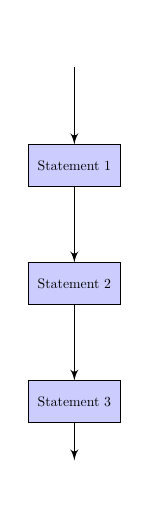
\begin{tikzpicture}[minimum height=1cm,auto,scale=0.50,transform shape]
    % Place nodes
    \node[draw=none] (start) {};
    \node [block, node distance=3cm,below of=start,text width=6em,minimum height=3em] (a) {Statement 1};
    \node [block, node distance=3cm,below of=a,text width=6em,minimum height=3em] (b) {Statement 2};
    \node [block, node distance=3cm,below of=b,text width=6em,minimum height=3em] (c) {Statement 3};
    \node[draw=none, below of=c,node distance=2cm] (end) {};
    % Draw edges
    \path [line] (start) -- (a);
    \path [line] (a) -- (b);
    \path [line] (b) -- (c);
    \path [line] (c) -- (end);
\end{tikzpicture}
\end{center}
\end{frame}

%\begin{frame}
%    \frametitle{Sequential Control Flow}
%    \framesubtitle{}
%
%\begin{center}
%\begin{tikzpicture}[minimum height=1cm,auto,scale=0.50,transform shape]
%    % Place nodes
%    \node[draw=none] (start) {};
%    \node [block, fill=red!20,node distance=3cm,below of=start,text width=6em,minimum height=3em] (a) {Statement 1};
%    \node [block, node distance=3cm,below of=a,text width=6em,minimum height=3em] (b) {Statement 2};
%    \node [block, node distance=3cm,below of=b,text width=6em,minimum height=3em] (c) {Statement 3};
%    \node[draw=none, below of=c,node distance=2cm] (end) {};
%    % Draw edges
%    \path [line] (start) -- (a);
%    \path [line] (a) -- (b);
%    \path [line] (b) -- (c);
%    \path [line] (c) -- (end);
%\end{tikzpicture}
%\end{center}
%\end{frame}
%
%\begin{frame}
%    \frametitle{Sequential Control Flow}
%    \framesubtitle{}
%
%\begin{center}
%\begin{tikzpicture}[minimum height=1cm,auto,scale=0.50,transform shape]
%    % Place nodes
%    \node[draw=none] (start) {};
%    \node [block, node distance=3cm,below of=start,text width=6em,minimum height=3em] (a) {Statement 1};
%    \node [block, fill=red!20,node distance=3cm,below of=a,text width=6em,minimum height=3em] (b) {Statement 2};
%    \node [block, node distance=3cm,below of=b,text width=6em,minimum height=3em] (c) {Statement 3};
%    \node[draw=none, below of=c,node distance=2cm] (end) {};
%    % Draw edges
%    \path [line] (start) -- (a);
%    \path [line] (a) -- (b);
%    \path [line] (b) -- (c);
%    \path [line] (c) -- (end);
%\end{tikzpicture}
%\end{center}
%\end{frame}
%
%\begin{frame}
%    \frametitle{Sequential Control Flow}
%    \framesubtitle{}
%
%\begin{center}
%\begin{tikzpicture}[minimum height=1cm,auto,scale=0.50,transform shape]
%    % Place nodes
%    \node[draw=none] (start) {};
%    \node [block, node distance=3cm,below of=start,text width=6em,minimum height=3em] (a) {Statement 1};
%    \node [block, node distance=3cm,below of=a,text width=6em,minimum height=3em] (b) {Statement 2};
%    \node [block, fill=red!20,node distance=3cm,below of=b,text width=6em,minimum height=3em] (c) {Statement 3};
%    \node[draw=none, below of=c,node distance=2cm] (end) {};
%    % Draw edges
%    \path [line] (start) -- (a);
%    \path [line] (a) -- (b);
%    \path [line] (b) -- (c);
%    \path [line] (c) -- (end);
%\end{tikzpicture}
%\end{center}
%
%\end{frame}

\subsection{Conditionals}

\begin{frame}
    \frametitle{If Statement Flow}
    \framesubtitle{}

\begin{center}

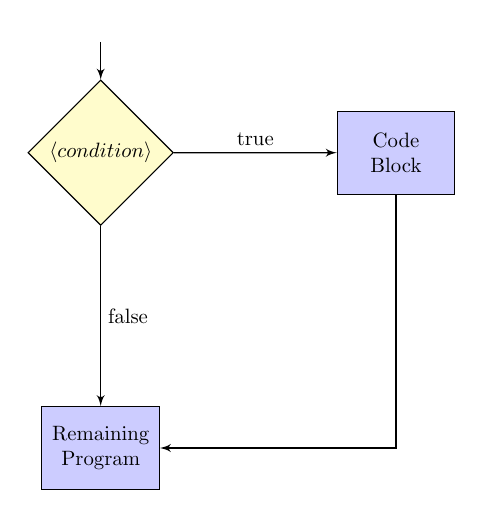
\begin{tikzpicture}[node distance = 4cm,auto,scale=0.75,transform shape]
    % Place nodes
    \node[draw=none] (start) {};
    \node [decision, below of=start,node distance=2cm] (decide) {$\langle condition \rangle$};
    \node [block, right of=decide] (a) {Code Block};
    \node[block,below of=decide] (c) {Remaining Program};
    % Draw edges
    \path [line] (start) -- (decide);
    \path [line] (decide) -- node {true}(a);
    \path [line] (decide) -- node {false}(c);
    \path [line] (a) |- (c);
\end{tikzpicture}

\end{center}

\end{frame}

%\begin{frame}
%    \frametitle{If Statement Flow}%2
%    \framesubtitle{}
%
%\begin{center}
%
%\begin{tikzpicture}[node distance = 4cm,auto,scale=0.75,transform shape]
%    % Place nodes
%    \node[draw=none] (start) {};
%    \node [decision,fill=red!20, below of=start,node distance=2cm] (decide) {$\langle condition \rangle$};
%    \node [block, right of=decide] (a) {Code Block};
%    \node[block,below of=decide] (c) {Remaining Program};
%    % Draw edges
%    \path [line] (start) -- (decide);
%    \path [line] (decide) -- node {true}(a);
%    \path [line] (decide) -- node {false}(c);
%    \path [line] (a) |- (c);
%\end{tikzpicture}
%
%\end{center}
%
%\end{frame}
%
%\begin{frame}
%    \frametitle{If Statement Flow}%3
%    \framesubtitle{}
%
%\begin{center}
%
%\begin{tikzpicture}[node distance = 4cm,auto,scale=0.75,transform shape]
%    % Place nodes
%    \node[draw=none] (start) {};
%    \node [decision, below of=start,node distance=2cm] (decide) {$\langle condition \rangle$};
%    \node [block, right of=decide,fill=red!20] (a) {Code Block};
%    \node[block,below of=decide] (c) {Remaining Program};
%    % Draw edges
%    \path [line] (start) -- (decide);
%    \path [line,red] (decide) -- node {true}(a);
%    \path [line] (decide) -- node {false}(c);
%    \path [line,red] (a) |- (c);
%\end{tikzpicture}
%
%\end{center}
%
%\end{frame}
%
%\begin{frame}
%    \frametitle{If Statement Flow}%4
%    \framesubtitle{}
%
%\begin{center}
%
%\begin{tikzpicture}[node distance = 4cm,auto,scale=0.75,transform shape]
%    % Place nodes
%    \node[draw=none] (start) {};
%    \node [decision, below of=start,node distance=2cm] (decide) {$\langle condition \rangle$};
%    \node [block, right of=decide] (a) {Code Block};
%    \node[block,below of=decide,fill=red!20] (c) {Remaining Program};
%    % Draw edges
%    \path [line] (start) -- (decide);
%    \path [line] (decide) -- node {true}(a);
%    \path [line,red] (decide) -- node {false}(c);
%    \path [line] (a) |- (c);
%\end{tikzpicture}
%
%\end{center}
%
%\end{frame}
%
\begin{frame}[fragile]
    \frametitle{If-Else Statement Flow}%1
    \framesubtitle{}

\begin{center}

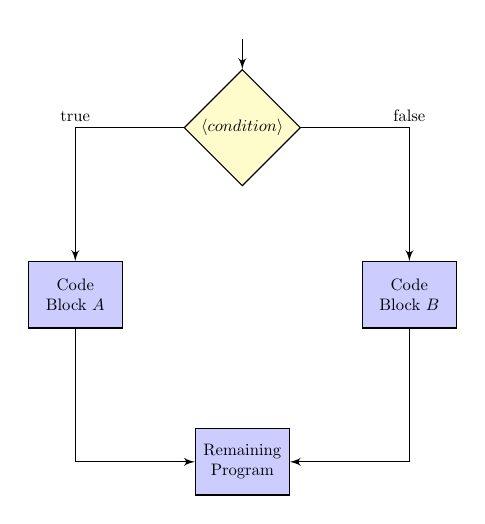
\begin{tikzpicture}[node distance = 4cm,auto,scale=0.60,transform shape]
    % Place nodes
    \node[draw=none] (start) {};
    \node [decision, below of=start,node distance=2cm] (decide) {$\langle condition \rangle$};
    \node [block, below left of=decide] (a) {Code Block $A$};
    \node [block, below right of=decide] (b) {Code Block $B$};
    \node[block,below left of=b] (c) {Remaining Program};
    % Draw edges
    \path [line] (start) -- (decide);
    \path [line] (decide) -| node[above] {true}(a);
    \path [line] (decide) -| node[above] {false}(b);
    \path [line] (a) |- (c);
    \path [line] (b) |- (c);
\end{tikzpicture}
\end{center}
\end{frame}
%
%\begin{frame}[fragile]
%    \frametitle{If-Else Statement Flow}%2
%    \framesubtitle{}
%
%\begin{center}
%
%\begin{tikzpicture}[node distance = 4cm,auto,scale=0.60,transform shape]
%    % Place nodes
%    \node[draw=none] (start) {};
%    \node [decision, fill=red!20,below of=start,node distance=2cm] (decide) {$\langle condition \rangle$};
%    \node [block, below left of=decide] (a) {Code Block $A$};
%    \node [block, below right of=decide] (b) {Code Block $B$};
%    \node[block,below left of=b] (c) {Remaining Program};
%    % Draw edges
%    \path [line] (start) -- (decide);
%    \path [line] (decide) -| node[above] {true}(a);
%    \path [line] (decide) -| node[above] {false}(b);
%    \path [line] (a) |- (c);
%    \path [line] (b) |- (c);
%\end{tikzpicture}
%\end{center}
%\end{frame}
%
%\begin{frame}[fragile]
%    \frametitle{If-Else Statement Flow}%3
%    \framesubtitle{}
%
%\begin{center}
%
%\begin{tikzpicture}[node distance = 4cm,auto,scale=0.60,transform shape]
%    % Place nodes
%    \node[draw=none] (start) {};
%    \node [decision, below of=start,node distance=2cm] (decide) {$\langle condition \rangle$};
%    \node [block, fill=red!20,below left of=decide] (a) {Code Block $A$};
%    \node [block, below right of=decide] (b) {Code Block $B$};
%    \node[block,below left of=b] (c) {Remaining Program};
%    % Draw edges
%    \path [line] (start) -- (decide);
%    \path [line,red] (decide) -| node[above] {true}(a);
%    \path [line] (decide) -| node[above] {false}(b);
%    \path [line,red] (a) |- (c);
%    \path [line] (b) |- (c);
%\end{tikzpicture}
%\end{center}
%\end{frame}
%
%\begin{frame}[fragile]
%    \frametitle{If-Else Statement Flow}%4
%    \framesubtitle{}
%
%\begin{center}
%
%\begin{tikzpicture}[node distance = 4cm,auto,scale=0.60,transform shape]
%    % Place nodes
%    \node[draw=none] (start) {};
%    \node [decision, below of=start,node distance=2cm] (decide) {$\langle condition \rangle$};
%    \node [block, below left of=decide] (a) {Code Block $A$};
%    \node [block, fill=red!20,below right of=decide] (b) {Code Block $B$};
%    \node[block,below left of=b] (c) {Remaining Program};
%    % Draw edges
%    \path [line] (start) -- (decide);
%    \path [line] (decide) -| node[above] {true}(a);
%    \path [line,red] (decide) -| node[above] {false}(b);
%    \path [line] (a) |- (c);
%    \path [line,red] (b) |- (c);
%\end{tikzpicture}
%\end{center}
%\end{frame}
%
%\begin{frame}[fragile]
%    \frametitle{If-Else Statement Flow}%5
%    \framesubtitle{}
%
%\begin{center}
%
%\begin{tikzpicture}[node distance = 4cm,auto,scale=0.60,transform shape]
%    % Place nodes
%    \node[draw=none] (start) {};
%    \node [decision, below of=start,node distance=2cm] (decide) {$\langle condition \rangle$};
%    \node [block, below left of=decide] (a) {Code Block $A$};
%    \node [block, below right of=decide] (b) {Code Block $B$};
%    \node[block,below left of=b,fill=red!20] (c) {Remaining Program};
%    % Draw edges
%    \path [line] (start) -- (decide);
%    \path [line] (decide) -| node[above] {true}(a);
%    \path [line] (decide) -| node[above] {false}(b);
%    \path [line] (a) |- (c);
%    \path [line] (b) |- (c);
%\end{tikzpicture}
%\end{center}
%\end{frame}

\begin{frame}
    \frametitle{If-Else-If Statement Flow}
    \framesubtitle{}

\begin{center}
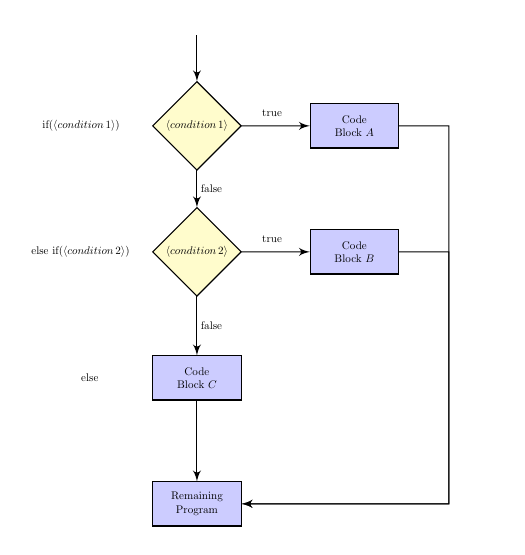
\begin{tikzpicture}[node distance=5cm,auto,scale=0.40,transform shape,every node/.style={text width=8em,minimum width=8em,minimum height=8em}]
    % Place nodes
    \node[draw=none,minimum height=0em] (start) {};
    \node [decision,below of=start,node distance=3cm] (condition1) {$\langle condition\,1 \rangle$};
    \node [decision,below of=condition1,node distance=4cm] (condition2) {$\langle condition\,2 \rangle$};

    \node [block, right of=condition1] (blockA) {Code Block $A$};
    \node [block, right of=condition2] (blockB) {Code Block $B$};
    \node [block, below of=condition2,node distance=4cm] (blockM) {Code Block $C$};

    \node[block,below of=blockM,node distance=4cm] (remaining) {Remaining Program};
    
    \node [left of=condition1,node distance=3.5cm,minimum width=10em] (code1) {if$\left(\langle condition\,1 \rangle\right)$};
    \node [left of=condition2,node distance=3.5cm,text width=10em] (code2) {else if$\left(\langle condition\,2 \rangle\right)$};
    \node [left of=blockM,node distance=3.5cm,text width=1em] (code5) {else};


    % Draw edges
    \path [line] (start) -- (condition1);
    \path [line] (condition1) -- node[pos=.95,yshift=-1cm] {true}(blockA);
    \path [line] (condition2) -- node[pos=.95,yshift=-1cm] {true}(blockB);
    
    \path [line] (condition1) -- node[pos=.5] {false}(condition2);
    \path [line] (condition2) -- node[pos=.5] {false}(blockM);
    \path [line] (blockM) -- node[pos=.5] {~}(remaining);

    \path [line] (blockA)   --++  (3,0) node [above] {~} |- (remaining);
    \path [line] (blockB)   --++  (3,0) node [above] {~} |- (remaining);

\end{tikzpicture}\end{center}

\end{frame}

\begin{frame}[plain]
    \frametitle{Generalized If-Else-If Statement Flow}
    \framesubtitle{}

\begin{center}
\vskip-1cm
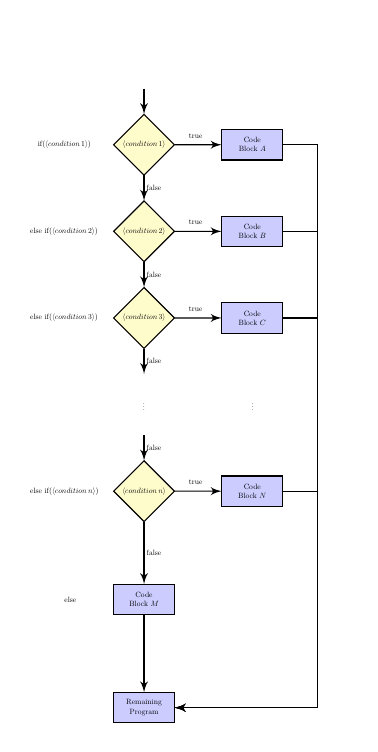
\begin{tikzpicture}[node distance=5cm,auto,scale=0.275,transform shape,every node/.style={text width=8em,minimum width=8em,minimum height=8em}]
    % Place nodes
    \node[draw=none] (start) {};
    \node [decision,below of=start,node distance=4cm] (condition1) {$\langle condition\,1 \rangle$};
    \node [decision,below of=condition1,node distance=4cm] (condition2) {$\langle condition\,2 \rangle$};
    \node [decision, below of=condition2,node distance=4cm] (condition3) {$\langle condition\,3 \rangle$};
    \node [decision,draw=none,fill=none, below of=condition3,node distance=4cm] (vdot1) {$\vdots$};
    \node [decision, below of=vdot1,node distance=4cm] (conditionX) {$\langle condition\,n \rangle$};

    \node [block, right of=condition1] (blockA) {Code Block $A$};
    \node [block, right of=condition2] (blockB) {Code Block $B$};
    \node [block, right of=condition3] (blockC) {Code Block $C$};
    \node [block,draw=none,fill=none, below of=blockC,node distance=4cm] (vdot2) {$\vdots$};
    \node [block, right of=conditionX] (blockN) {Code Block $N$};
    \node [block, below of=conditionX] (blockM) {Code Block $M$};

    \node[block,below of=blockM] (remaining) {Remaining Program};
    
    \node [left of=condition1,node distance=3.5cm,minimum width=10em] (code1) {if$\left(\langle condition\,1 \rangle\right)$};
    \node [left of=condition2,node distance=3.5cm,text width=10em] (code2) {else if$\left(\langle condition\,2 \rangle\right)$};
    \node [left of=condition3,node distance=3.5cm,text width=10em] (code3) {else if$\left(\langle condition\,3 \rangle\right)$};
    \node [left of=conditionX,node distance=3.5cm,text width=10em] (code4) {else if$\left(\langle condition\,n \rangle\right)$};
    \node [left of=blockM,node distance=3.5cm,text width=1em] (code5) {else};


    % Draw edges
    \path [line] (start) -- (condition1);
    \path [line] (condition1) -- node[pos=.95,yshift=-1cm] {true}(blockA);
    \path [line] (condition2) -- node[pos=.95,yshift=-1cm] {true}(blockB);
    \path [line] (condition3) -- node[pos=.95,yshift=-1cm] {true}(blockC);
    \path [line] (conditionX) -- node[pos=.95,yshift=-1cm] {true}(blockN);
    
    \path [line] (condition1) -- node[pos=.5] {false}(condition2);
    \path [line] (condition2) -- node[pos=.5] {false}(condition3);
    \path [line] (condition3) -- node[pos=.5] {false}(vdot1);
    \path [line] (vdot1) -- node[pos=.5] {false}(conditionX);
    \path [line] (conditionX) -- node[pos=.5] {false}(blockM);
    \path [line] (blockM) -- node[pos=.5] {~}(remaining);

    \path [line] (blockA)   --++  (3,0) node [above] {~} |- (remaining);
    \path [line] (blockB)   --++  (3,0) node [above] {~} |- (remaining);
    \path [line] (blockC)   --++  (3,0) node [above] {~} |- (remaining);
    \path [line] (blockN)   --++  (3,0) node [above] {~} |- (remaining);

%    \path [line] (b) -- (c);
\end{tikzpicture}\end{center}

\end{frame}

\subsection{Boolean Statements}

\begin{frame}
    \frametitle{Boolean Statements}
    \framesubtitle{}

\begin{itemize}[<+->]
  \item A \emph{boolean} condition or expression is a logical expression that evaluates to either \emph{true} or \emph{false}
  \item May involve numerical comparisons $a \geq 0$
  \item A condition can be \emph{simple} or \emph{complex}
  \item May connect one or more expressions using a logical \emph{and} or a logical \emph{or}
\end{itemize}

\end{frame}

\subsection{Numeric Comparisons}

\begin{frame}[fragile]
  \frametitle{Numeric Comparisons}
  \framesubtitle{}

\begin{itemize}[<+->]
  \item We need a way to compare the value stored in variables
  \item Compare the relative value of two variables
  \item Compare the value stored in one variable with a fixed value (literal)
  \item Comparisons:
  \begin{itemize}
    \item Are two values equal or not equal?
    \item Is one value greater than or equal to/lesser than or equal to another?
    \item Is one value strictly greater/lesser than another?
  \end{itemize}
  \item Standard mathematical notations
  	$$= \quad \neq \quad \geq \quad \leq \quad  > \quad <$$
  \item Code versions:
  \begin{center}
  	\mintinline{c}{==   !=   >=   <=   >   <}
  \end{center}
\end{itemize}

\end{frame}

\subsection{Complex Logic Statements}
  %AND, OR, Negation

\begin{frame}[fragile]
    \frametitle{Logical And}
    \framesubtitle{}
    
    \begin{center}
    \begin{tabular}{c|c|c}
    $A$ & $B$ & $A$ \emph{and} $B$ \\
    \hline\hline
    false & false & false\\
    false & true & false\\
    true & false & false\\
    true & true & true\\
    \end{tabular}
    \end{center}

\onslide<2->{Code version: \mintinline{c}{&&}}
\end{frame}

\begin{frame}
    \frametitle{Logical Or}
    \framesubtitle{}

    \begin{center}
    \begin{tabular}{c|c|c}
    $A$ & $B$ & $A$ \emph{or} $B$ \\
    \hline\hline
    false & false & false\\
    false & true & true\\
    true & false & true\\
    true & true & true\\
    \end{tabular}
    \end{center}
    
\onslide<2->{Code version: \mintinline{c}{||}}
    
\end{frame}

\begin{frame}
    \frametitle{Logical Negation}
    \framesubtitle{}

    \begin{center}
    \begin{tabular}{c|c}
    $A$  & \emph{not} $A$ \\
    \hline\hline
    false & true\\
    true & false\\
    \end{tabular}
    \end{center}

\onslide<2->{Code version: \mintinline{c}{!}}
    
\end{frame}

  
\section{Conditionals}

\begin{frame}
    \frametitle{}
    \framesubtitle{}
    
    \begin{center}
    {\Huge Part II: Conditionals}\\
    {\Large If, If-Else, If-Else-If \& Numeric Comparisons}
    \end{center}

%TODO: if, if-else, if-else-if and numeric comparisons
%example: huskers win/lose/tie

\end{frame}

\begin{frame}[fragile]
    \frametitle{If Statement}
    \framesubtitle{}

\begin{minted}{c}
if(<condition>) {
  //conditional body: code inside this code block
  //will only execute if the <condition> evaluates
  //to true, otherwise it will not execute at all
}
\end{minted}    

\begin{itemize}[<+->]
  \item Uses the keyword \mintinline{c}{if}
  \item The condition is enclosed in parentheses
  \item The code block begins and ends with curly brackets
  \item Behavior
\end{itemize}

\end{frame}

\begin{frame}[fragile]
    \frametitle{If-Else Statement}
    \framesubtitle{}

\begin{minted}{c}
if(<condition>) {
  //code block A
} else {
  //code block B
}
\end{minted}    

\begin{itemize}[<+->]
  \item Uses the keyword \mintinline{c}{else}
  \item Behavior: if \mintinline{c}{<condition>} evaluates to true
  code block \mintinline{c}{A} is executed
  \item If \mintinline{c}{<condition>} evaluates to false, 
  code block \mintinline{c}{B} is executed
  \item The two code blocks are \emph{mutually exclusive}
  \item A generalization of the \mintinline{c}{if} statement
\end{itemize}

\end{frame}

\begin{frame}[fragile]
    \frametitle{If-Else-If Statement}
    \framesubtitle{}

\begin{minted}{c}
if(<condition1>) {
  //code block A
} else if(<condition2>) {
  //code block B
} else {
  //code block C
}
\end{minted}    

\vskip-1cm
\begin{itemize}[<+->]
  \item Multiple conditions: may define as many as you want
  \item The \emph{first} condition that evaluates to true is the one (and only one) that is executed
  \item Each code block is \emph{mutually exclusive}
  \item The most specific conditions come \emph{first}, more general \emph{last}
  \item You may omit the final \mintinline{c}{else} block if there is no ``final case'' to consider
\end{itemize}

\end{frame}

\subsection{Numerical Comparisons}

\begin{frame}[fragile]
  \frametitle{Numerical Comparisons}
  \framesubtitle{}

\begin{itemize}[<+->]
  \item Comparison operators: \\
  \mintinline{c}{<}, \mintinline{c}{>}, \mintinline{c}{<=}, \mintinline{c}{>=}
  \item Equality operator: \mintinline{c}{==}
  \item Inequality operators \mintinline{c}{!=}
  \item May be used in combinations of \emph{literals} (hardcoded numerical values), variables or expressions
\end{itemize}

\end{frame}

\begin{frame}[fragile]
  \frametitle{Numerical Comparisons}
  \framesubtitle{}

%TODO: type this out in a demo instead of slide
\begin{minted}[fontsize=\tiny]{c}
int a, b, c;

//comparing a variable to a literal
if(a == 0) {
  printf("a is zero!\n");
}

//comparing two variable values:
if(a == b) {
  printf("the two values are equal\n");
}

//you can, but shouldn't do the following
if(10 == a) {
 //...
}

if(b * b - 4 * a * c < 0) {
 printf("looks bad...\n");
}

//you can but shouldn't:
if(10 < 20) {
 printf("duh, that's always true\n");
}
\end{minted}
\end{frame}

\subsection{Examples}

\begin{frame}[fragile]
  \frametitle{Conditional Examples}
  \framesubtitle{}

%TODO: type this out in a demo instead of slide
\begin{minted}[fontsize=\tiny]{c}
int huskerScore;
int opponentScore;

//a simple if statement:
if(huskerScore > opponentScore) {
  printf("Huskers Win!\n");
}

//an if-else statement:
if(huskerScore > opponentScore) {
  printf("Huskers Win!\n");
} else {
  printf("Huskers do not win.\n");
}

//an if-else-if statement:
if(huskerScore > opponentScore) {
  printf("Huskers Win!\n");
} else if(huskersScore < opponentScore) {
  printf("Huskers Lose!\n");
} else {
  printf("Tie, let's go to overtime!\n");
}
\end{minted}
\end{frame}


\begin{frame}[fragile]
  \frametitle{Coding Style}
  \framesubtitle{}

\begin{columns}[T] % align columns
\begin{column}{.60\textwidth}
\begin{minted}[fontsize=\footnotesize]{c}
if(huskerScore > opponentScore) {
  printf("Huskers Win!\n");
} else if(huskersScore < opponentScore) {
  printf("Huskers Lose!\n");
} else {
  printf("Tie, let's go to overtime!\n");
}
\end{minted}
\end{column}%
\hfill
\begin{column}{.4\textwidth}
{\footnotesize
\begin{itemize}[<+->]
  \item Use of spaces
  \item Opening curly brackets on the same line as keywords
  \item Closing curly brackets on the same indentation level
  \item All blocks are indented at the same level
  \item Consistency is the most important thing
\end{itemize}
}
\end{column}%
\end{columns}


\end{frame}


\section{Logical Operators}

\subsection{Negation}
 %Negation, AND, OR
\begin{frame}
    \frametitle{}
    \framesubtitle{}
    
    \begin{center}
    {\Huge Part III: Logical Operators}\\
    {\Large Negation, Logical And, Logical Or}
    \end{center}

\end{frame}

\begin{frame}[fragile]
  \frametitle{Negation Operator}
  \framesubtitle{}

\begin{itemize}[<+->]
  \item Any logical statement can be negated using \mintinline{c}{!}
  \item Negation of \mintinline{c}{(a == b)} can be \mintinline{c}{!(a == b)}
  \item Negation of \mintinline{c}{(a <= b)} can be \mintinline{c}{!(a <= b)}
  \item Better to use: \mintinline{c}{(a != b)} and \mintinline{c}{(a > b)}
  \item Usually a negation is used on a ``flag'' variable: a variable that simply holds a truth value (true or false)
\end{itemize}

\end{frame}

\subsection{Flag Variables}

\begin{frame}[fragile]
  \frametitle{Flag Variables}
  \framesubtitle{}

\begin{itemize}[<+->]
  \item C has no ``boolean variables''
  \item Any numerical value can be treated as a boolean value 
  \item \mintinline{c}{0} is false
  \item Any non-zero value is true
  \item \mintinline{c}{3, 3.5, 3.14, -10} are all true
  \item Convention: use \mintinline{c}{1} as true
  \item Best practice: only use \mintinline{c}{int} variables as booleans
\end{itemize}

\end{frame}

\begin{frame}[fragile]
  \frametitle{Flag Variables}
  \framesubtitle{Example}
  
\begin{minted}[fontsize=\footnotesize]{c}
//flag variable to indicate if someone is a 
//student (true) or not (false)
int isStudent;

//set the variable to true:
isStudent = 1;

//they are not a student:
isStudent = 0;

if(isStudent) {
  printf("You get a student discount!\n");
}

//using a negation
if(!isStudent) {
  printf("You pay full price!\n");
}
\end{minted}

\end{frame}

\subsection{Logical And}

\begin{frame}[fragile]
  \frametitle{Logical And}
  \framesubtitle{}
  
\begin{itemize}[<+->]
  \item Logical And operator: \mintinline{c}{&&}
  \item Evaluates to true only if \emph{both} operands evaluate to true
\end{itemize}

\begin{overprint}
\onslide<3>
\begin{minted}{c}
if(subTotal >= 50.0 && isPreferredMember) {
  discount = .20;
  shipping = 0;
} else if(subTotal >= 50.0 && !isPreferredMember) {
  discount = 0.0;
  shipping = 0;
} else {
  discount = 0.0;
  shipping = 10.50;
}
\end{minted}
\end{overprint}
\end{frame}

\subsection{Logical Or}

\begin{frame}[fragile]
  \frametitle{Logical Or}
  \framesubtitle{}
  
\begin{itemize}[<+->]
  \item Logical Or operator: \mintinline{c}{||}
  \item Evaluates to true only if \emph{at least one} of its operands evaluate to true
\end{itemize}

\begin{overprint}
\onslide<3>
\begin{minted}{c}
if(isStudent || isPreferredMember) {
  discount = .20;
}
\end{minted}
\end{overprint}

\end{frame}

\subsection{Examples}

\begin{frame}[fragile]
  \frametitle{Examples}
  \framesubtitle{}

\begin{minted}{c}
if(a > 10 && a < 20) {
  //...
}

if(a == b && a < 10) {
  //...
}

if(a > 10 || a < 20) {
  //...
}

if(a == b || a < 10) {
  //...
}
\end{minted}

\end{frame}

\section{Pitfalls}

\begin{frame}
    \frametitle{}
    \framesubtitle{}
    
    \begin{center}
    {\Huge Part IV: Pitfalls}\\
    {\Large Common Errors \& Misconceptions}
    \end{center}

\end{frame}


\begin{frame}[fragile]
  \frametitle{Pitfall}
  \framesubtitle{Incorrect Complex Logic}

Consider the following code:

\begin{minted}{c}
if(0 <= a <= 10) {
  printf("Value is within range!\n");
}
\end{minted}

\begin{itemize}[<+->]
  \item The above code will compile, will execute, but will 
    not work for certain values
  \item What happens when \mintinline{c}{a = 20}?
  \item First comparison: \mintinline{c}{0 <= 20}
  \item Evaluates to true (\mintinline{c}{1})
  \item Second comparison: \mintinline{c}{1 <= 10} (true)
  \item Incorrect result
\end{itemize}
\end{frame}

\begin{frame}[fragile]
  \frametitle{Pitfall}
  \framesubtitle{Incorrect Complex Logic}

Solution: break up your conditions using a \mintinline{c}{&&}

\begin{minted}{c}
if(0 <= a && a <= 10) {
  printf("Value is within range!\n");
}
\end{minted}

\end{frame}

\begin{frame}[fragile]
  \frametitle{Pitfall}
  \framesubtitle{Confusing Comparisons \& Assignments}

Consider the following code:

\begin{minted}{c}
int a = 5;

if(a = 10) {
  printf("a is ten\n");
}
\end{minted}

\begin{itemize}[<+->]
  \item The above code will compile, run, but will give incorrect results
  \item \mintinline{c}{a = 10} results in an assignment of the value 10 to the variable \mintinline{c}{a}
  \item A value of 10 evaluates to true
  \item The \mintinline{c}{if} body gets executed regardless of the original value of 
  \mintinline{c}{a}
\end{itemize}

\end{frame}

\begin{frame}[fragile]
  \frametitle{Pitfall}
  \framesubtitle{Improper Semicolons}

Consider the following code:

\begin{minted}{c}
int a = 5;

if(a == 10); {
  printf("a is ten!\n");
}
\end{minted}

\begin{itemize}[<+->]
  \item Semicolon (in general) only go after \emph{executable} statements
  \item Above code will compile, will run, but will not give the correct results
  \item Conditional statement is \emph{bound} to an empty statement
\end{itemize}

\end{frame}

\subsection{Non-Numerical Comparisons}

\begin{frame}[fragile]
  \frametitle{Non-Numerical Comparisons}
  \framesubtitle{~}

\begin{itemize}[<+->]
  \item You can compare single \mintinline{c}{char} values with character literals:
  
\begin{minted}{c}
char initial = 'C';

if(initial == 'c' || initial == 'C') {
  //...
}
\end{minted}

\item You \emph{cannot} use equality and inequality operators on strings (sequences of characters)

\begin{minted}{c}
if(name == "Chris") {
  printf("Greetings, Professor.\n");
}
\end{minted}
\item The above will \emph{never} give correct results
\end{itemize}

\end{frame}

\subsection{Precedence Rules}

\begin{frame}[fragile]
  \frametitle{Precedence Rules}
  \framesubtitle{~}

\begin{itemize}[<+->]
  \item The logical \emph{and} \mintinline{c}{&&} is evaluated before
  the logical \emph{or} \mintinline{c}{||}
  \item The following are \emph{not} equivalent:\\  
  \mintinline{c}{a && (b || c)} \\
  \mintinline{c}{a && b || c}
  \item Use parentheses when necessary
  \item Best practice: use them even when not necessary to express \emph{intent}
\end{itemize}

\end{frame}


\subsection{Short Circuiting}

\begin{frame}[fragile]
  \frametitle{Short-Circuiting}
  \framesubtitle{~}

Consider a logical and: \mintinline{c}{a && b}

\begin{itemize}[<+->]
  \item If \mintinline{c}{a} evaluates to false, it does not matter 
  what \mintinline{c}{b} evaluates to
  \item Since \mintinline{c}{a} is false, the entire expression is false
  \item Consequently: \mintinline{c}{b} is not evaluated/executed
\end{itemize}

\end{frame}

\begin{frame}[fragile]
  \frametitle{Short-Circuiting}
  \framesubtitle{~}

Consider a logical and: \mintinline{c}{a || b}    
\begin{itemize}[<+->]
  \item If \mintinline{c}{a} evaluates to true, it does not matter 
  what \mintinline{c}{b} evaluates to
  \item Since \mintinline{c}{a} is true, the entire expression is true
  \item Consequently: \mintinline{c}{b} is not evaluated/executed
\end{itemize}

\end{frame}

\begin{frame}[fragile]
  \frametitle{Short-Circuiting}
  \framesubtitle{~}

\begin{itemize}[<+->]
  \item Short circuiting is common to the vast majority of programming language
  \item Historic reasons
  \item Common \emph{idiom} in many programming languages:
\end{itemize}

\begin{overprint}
\onslide<3>
\begin{minted}{c}
if(a != NULL && a[0] == 10) {
  //...
}
\end{minted}
\end{overprint}

\end{frame}

%\begin{frame}[fragile]
%  \frametitle{Short-Circuiting}
%
%Evaluation Tree of \mintinline{c}{A && B || C}
%
%\begin{center}
%\begin{tikzpicture}[node distance = 5cm, auto,scale=1.0,transform shape]
%    \node {\mintinline{c}{||}}
%      child {node {\mintinline{c}{&&}}
%        child {node {\mintinline{c}{A}}}
%        child {node {\mintinline{c}{B}}}
%      }
%      child {node {\mintinline{c}{C}}};
%\end{tikzpicture}
%\end{center}
%
%\end{frame}
%
%\begin{frame}[fragile]
%  \frametitle{Short-Circuiting}
%
%Evaluation Tree of \mintinline{c}{A || B && C}
%
%\begin{center}
%\begin{tikzpicture}[node distance = 5cm, auto,scale=1.0,transform shape]
%    \node {\mintinline{c}{||}}
%      child {node {\mintinline{c}{&&}}
%        child {node {\mintinline{c}{A}}}
%        child {node {\mintinline{c}{B}}}
%      }
%      child {node {\mintinline{c}{C}}};
%\end{tikzpicture}
%\end{center}
%
%\end{frame}

 
\section{Exercises}

\begin{frame}
    \frametitle{}
    \framesubtitle{}
    
    \begin{center}
    {\Huge Part V: Exercises}\\
    {\Large ~}
    \end{center}

\end{frame}

\begin{frame}
  \frametitle{Exercise}
  \framesubtitle{}
  
  Write a code snippet that determines the maximum of three integer
  values.

\end{frame}

\begin{frame}
  \frametitle{Exercise}
  \framesubtitle{}

Write a program that reads a decibel level from the user
and gives them a description of the sound level based on
the following categories.

\begin{itemize}
  \item 0 - 60 Quiet
  \item 61 - 70 Conversational
  \item 71 - 90 Loud
  \item 91 - 110 Very Loud
  \item 111 - 129 Dangerous
  \item 130 - 194 Very Dangerous
  %\item < 0 or 195+
\end{itemize}

\end{frame}


\begin{frame}
  \frametitle{Exercise}
  \framesubtitle{}

%A triangle can be characterized in terms of the length of its three sides.  
%In particular, an equilateral triangle is a triangle with all three sides being 
%equal.  A triangle such that two sides have the same length is isosceles 
%and a triangle with all three sides having a different length is scalene.  
%Examples of each can be found in Figure \ref{fig:triangles}.

\begin{figure}[h]
\centering

\includegraphics[scale=0.25]{images/triangleEquilateral}~~~~~~~

\includegraphics[scale=0.250]{images/triangleIsosceles}~~~~~~~

\includegraphics[scale=0.250]{images/triangleScalene}
\caption{Examples of Equilateral, Isosceles, and Scalene triangles}
\label{fig:triangles}
\end{figure}

3 sides are a valid triangle only if the sum of the 
length of any two sides is strictly greater than the length of the third side.  

Write a program to determine if 3 inputs form a valid triangle and if so,
what type.

%In this exercise you will complete a program that determines if 3 values 
%form a valid triangle.  If valid, the program should output whether or not 
%the triangle is equilateral, isosceles or scalene.  The program has been 
%started for you (see \mintinline{text}{triangles.c}), which reads in the three sides of a 
%triangle via command line arguments.  Complete the program by 
%implementing the logic to determine if the sides form a valid triangle 
%and if so, what type.
%
%After you have completed the program and thoroughly tested it, hand 
%it in using webhandin and grade yourself using webgrader.  Refer to 
%the previous lab for instructions on how to do this if you've forgotten.  
%Demonstrate your graded program to a lab instructor and have them 
%sign your worksheet.


\end{frame}



\end{document} 
